\documentclass{article}

% Margins
\usepackage[top=2.5cm, left=3cm, right=3cm, bottom=4.0cm]{geometry}
\geometry{legalpaper, portrait, margin=1.25in}
\usepackage[english]{babel}
\usepackage[utf8]{inputenc}
\usepackage{amsmath,amssymb}
\usepackage{parskip}
\usepackage{graphicx}
\usepackage{float} % For [H] option
\usepackage{placeins}
\usepackage{listings}
\usepackage{color}

\definecolor{dkgreen}{rgb}{0,0.6,0}
\definecolor{gray}{rgb}{0.5,0.5,0.5}
\definecolor{mauve}{rgb}{0.58,0,0.82}

\lstset{frame=tb,
	language=R,
	aboveskip=3mm,
	belowskip=3mm,
	showstringspaces=false,
	columns=flexible,
	basicstyle={\small\ttfamily},
	numbers=none,
	numberstyle=\tiny\color{gray},
	keywordstyle=\color{blue},
	commentstyle=\color{dkgreen},
	stringstyle=\color{mauve},
	breaklines=true,
	breakatwhitespace=true,
	tabsize=3
}
% Colour table cells
% \usepackage[table]{xcolor}

% Get larger line spacing in table
\newcommand{\tablespace}{\\[1.25mm]}
\newcommand\Tstrut{\rule{0pt}{2.6ex}}         % = `top' strut
\newcommand\tstrut{\rule{0pt}{2.0ex}}         % = `top' strut
\newcommand\Bstrut{\rule[-0.9ex]{0pt}{0pt}}   % = `bottom' strut

%%%%%%%%%%%%%%%%%
%     Title     %
%%%%%%%%%%%%%%%%%
\title{\vspace{-30}Assignment tasks for the \textit{Junior Quantitative Analyst in Immigration Research} position}
\author{Candidate: Lorenzo Gorini\\Immigration Policy Lab (ETH)}
\date{\vspace{-10}\today}

\begin{document}
	\maketitle
	\section{Question 1: Job episodes}
	In order to find the solution, I first made few assumptions on the dataset:
	\begin{enumerate}
		\item YM\_start of a job is always before the YM\_end of the same job
		\item The person never started a job in the country before getting in the
		country. This means that YM\_start of a job is always after the YM\_in of
		the same person
		\item The person never started a job in the country after leaving the
		country. This means that YM\_start and YM\_end of a job is always before
		the YM\_out
		\item The person never had multiple jobs contemporarily
	\end{enumerate}
	
	On the contrary, I found out that assumptions 2 to 4 are wrong. So I handled the inconsistencies related to 2. and 3. Regarding the assumption n.4, I assumed that it was possible for a person to have multiple jobs contemporarily. 
	So, for example, if that person had 2 jobs in the same month, I counted as if he/she had worked 2 months. On the other hand, since we want to compare the number of months worked by immigrants in the first 3 years, I capped their total months worked to 3*12=36 months. The total number of immigrants that, based on this computation, worked more than 36 months worked are 56.
	
	The result of my analysis is shown in the Fig. \ref{fig:total_months_per_pers_histogram} and Fig. \ref{fig:total_months_per_pers_violin_plot}
	Particularly, the mean of months worked by immigrants in the first 3 years, since they entered the country, is 5.1189 months.  The median is 0 months, and the maximum is 36. 
	On the other hand, the maximum is 162 months when their total months worked are not capped to 36).
	\begin{figure}[H]\centering
		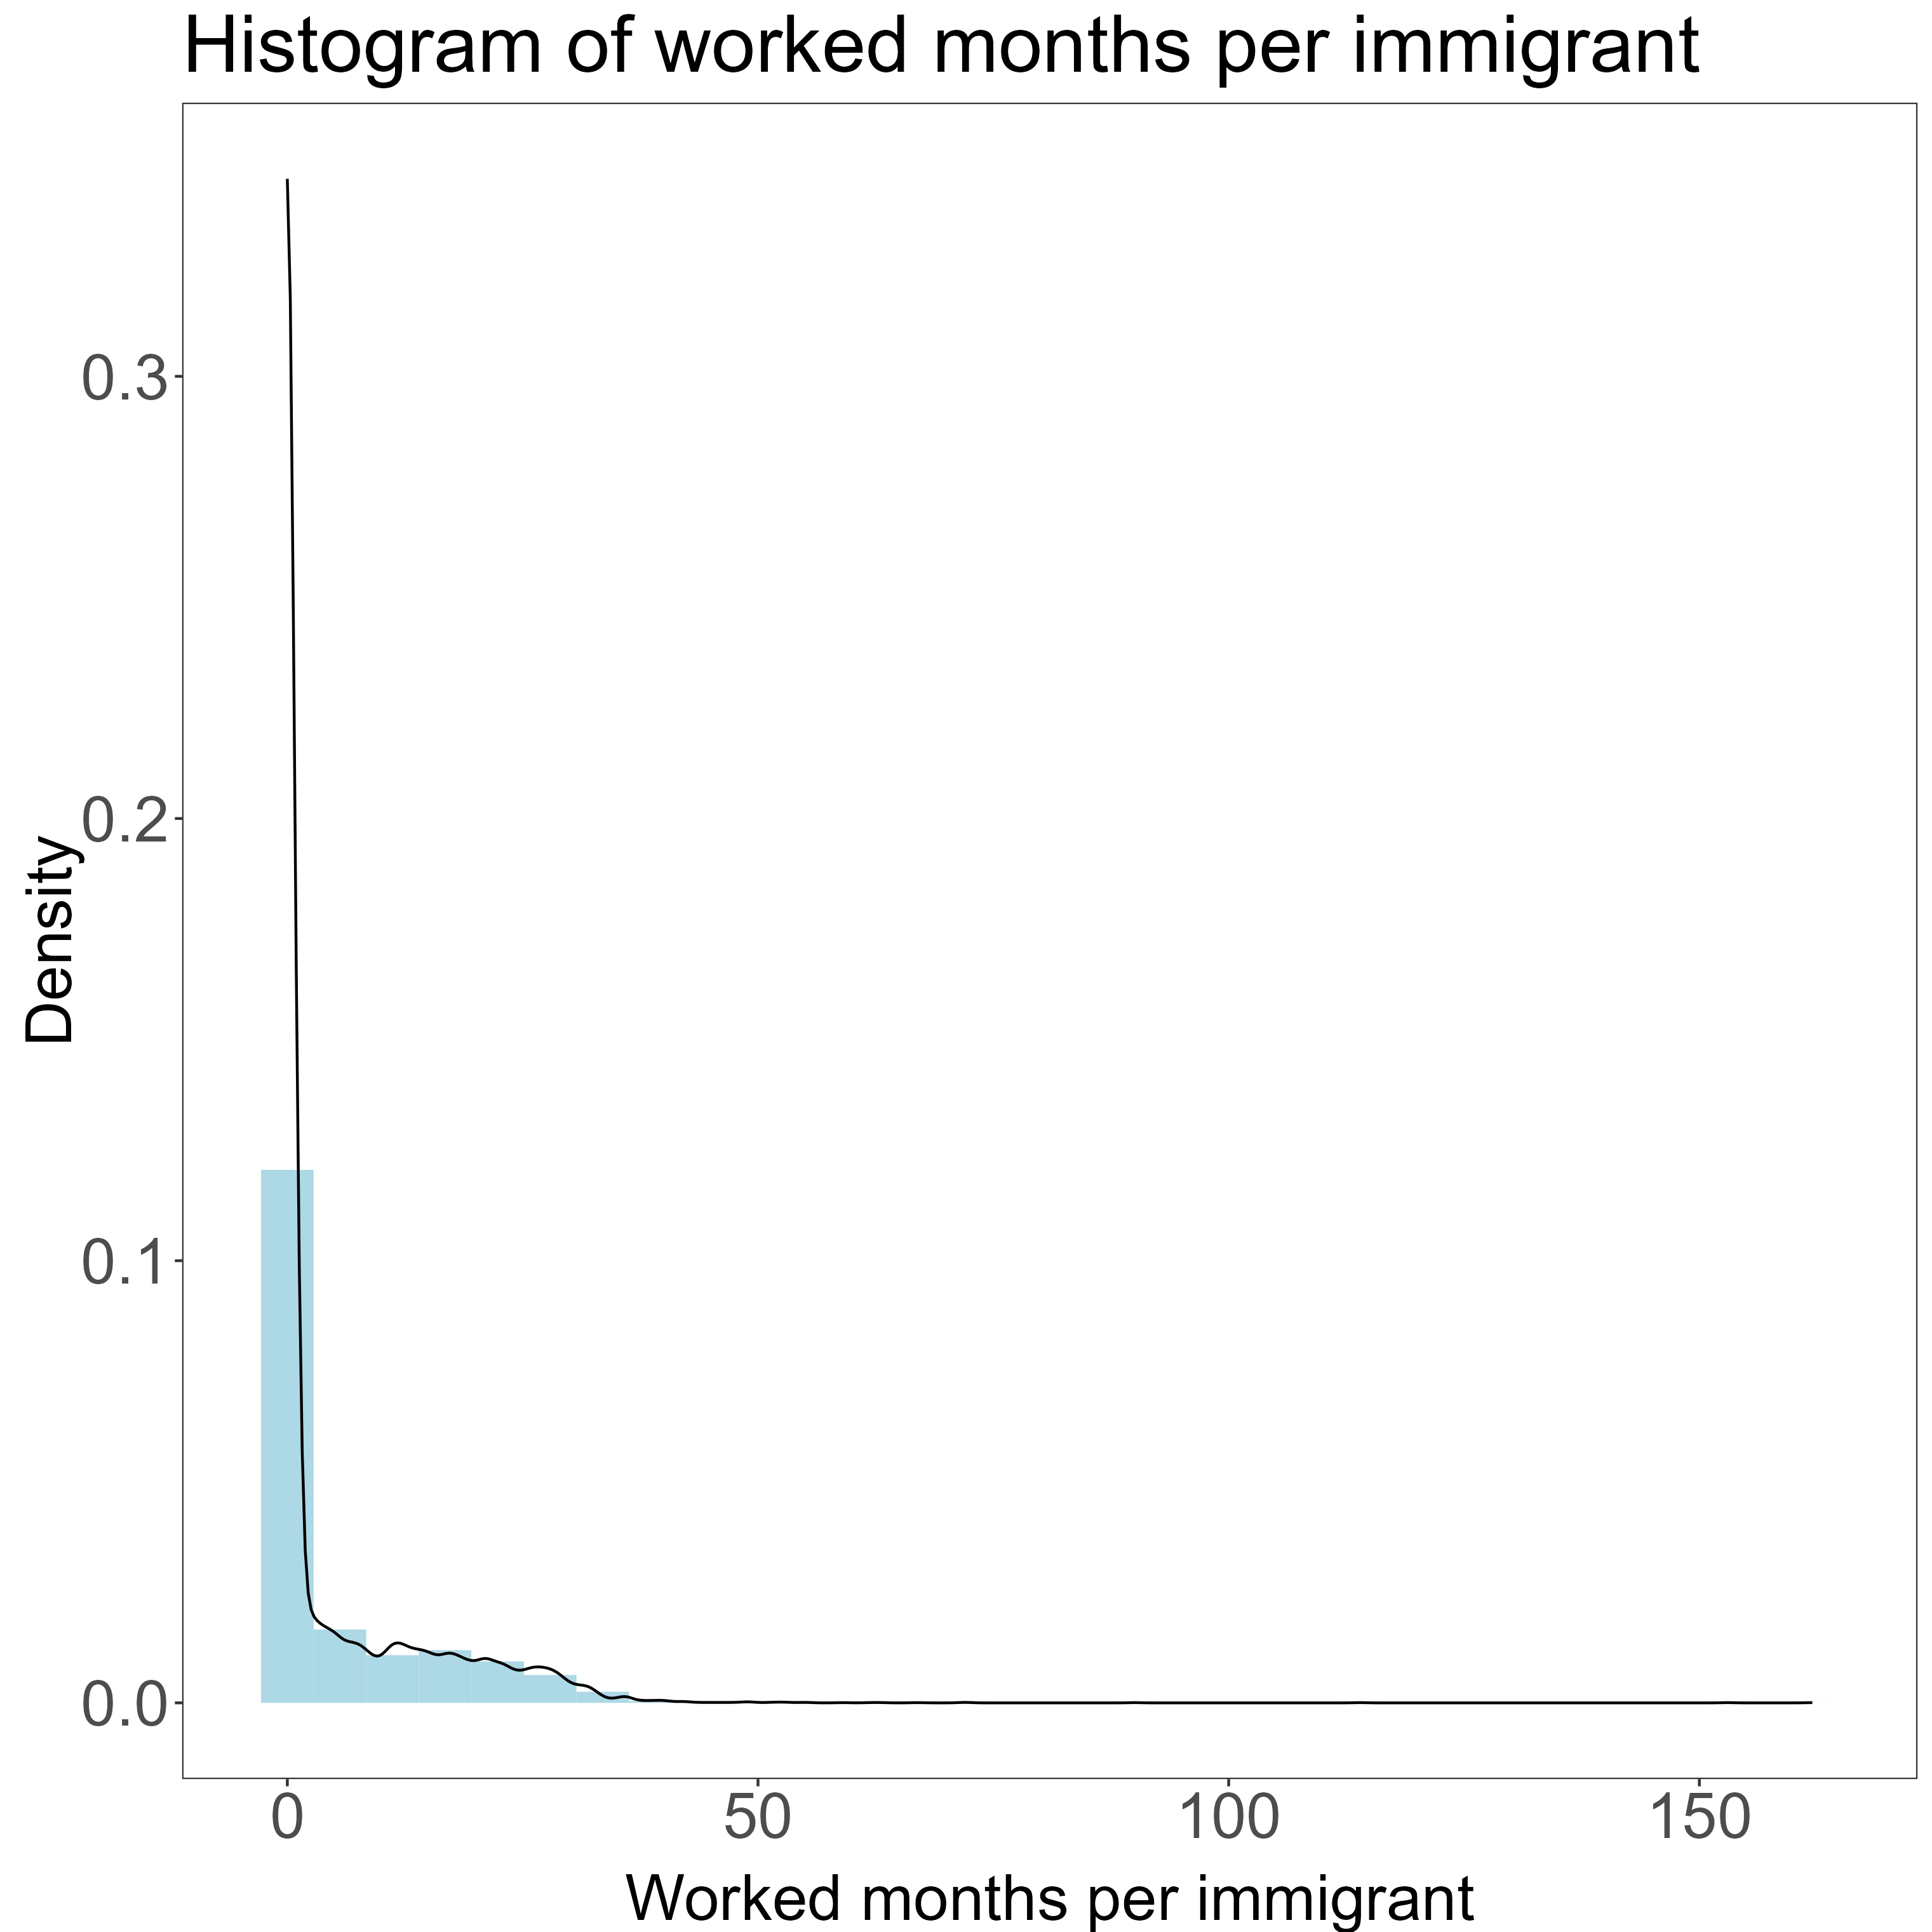
\includegraphics[width=10cm]{total_months_per_pers_histogram}
		\caption{Histogram showing the distribution of months worked by immigrants in the first 3 years, since they entered the country.}
		\label{fig:total_months_per_pers_histogram}
	\end{figure}
	\begin{figure}[H]\centering
		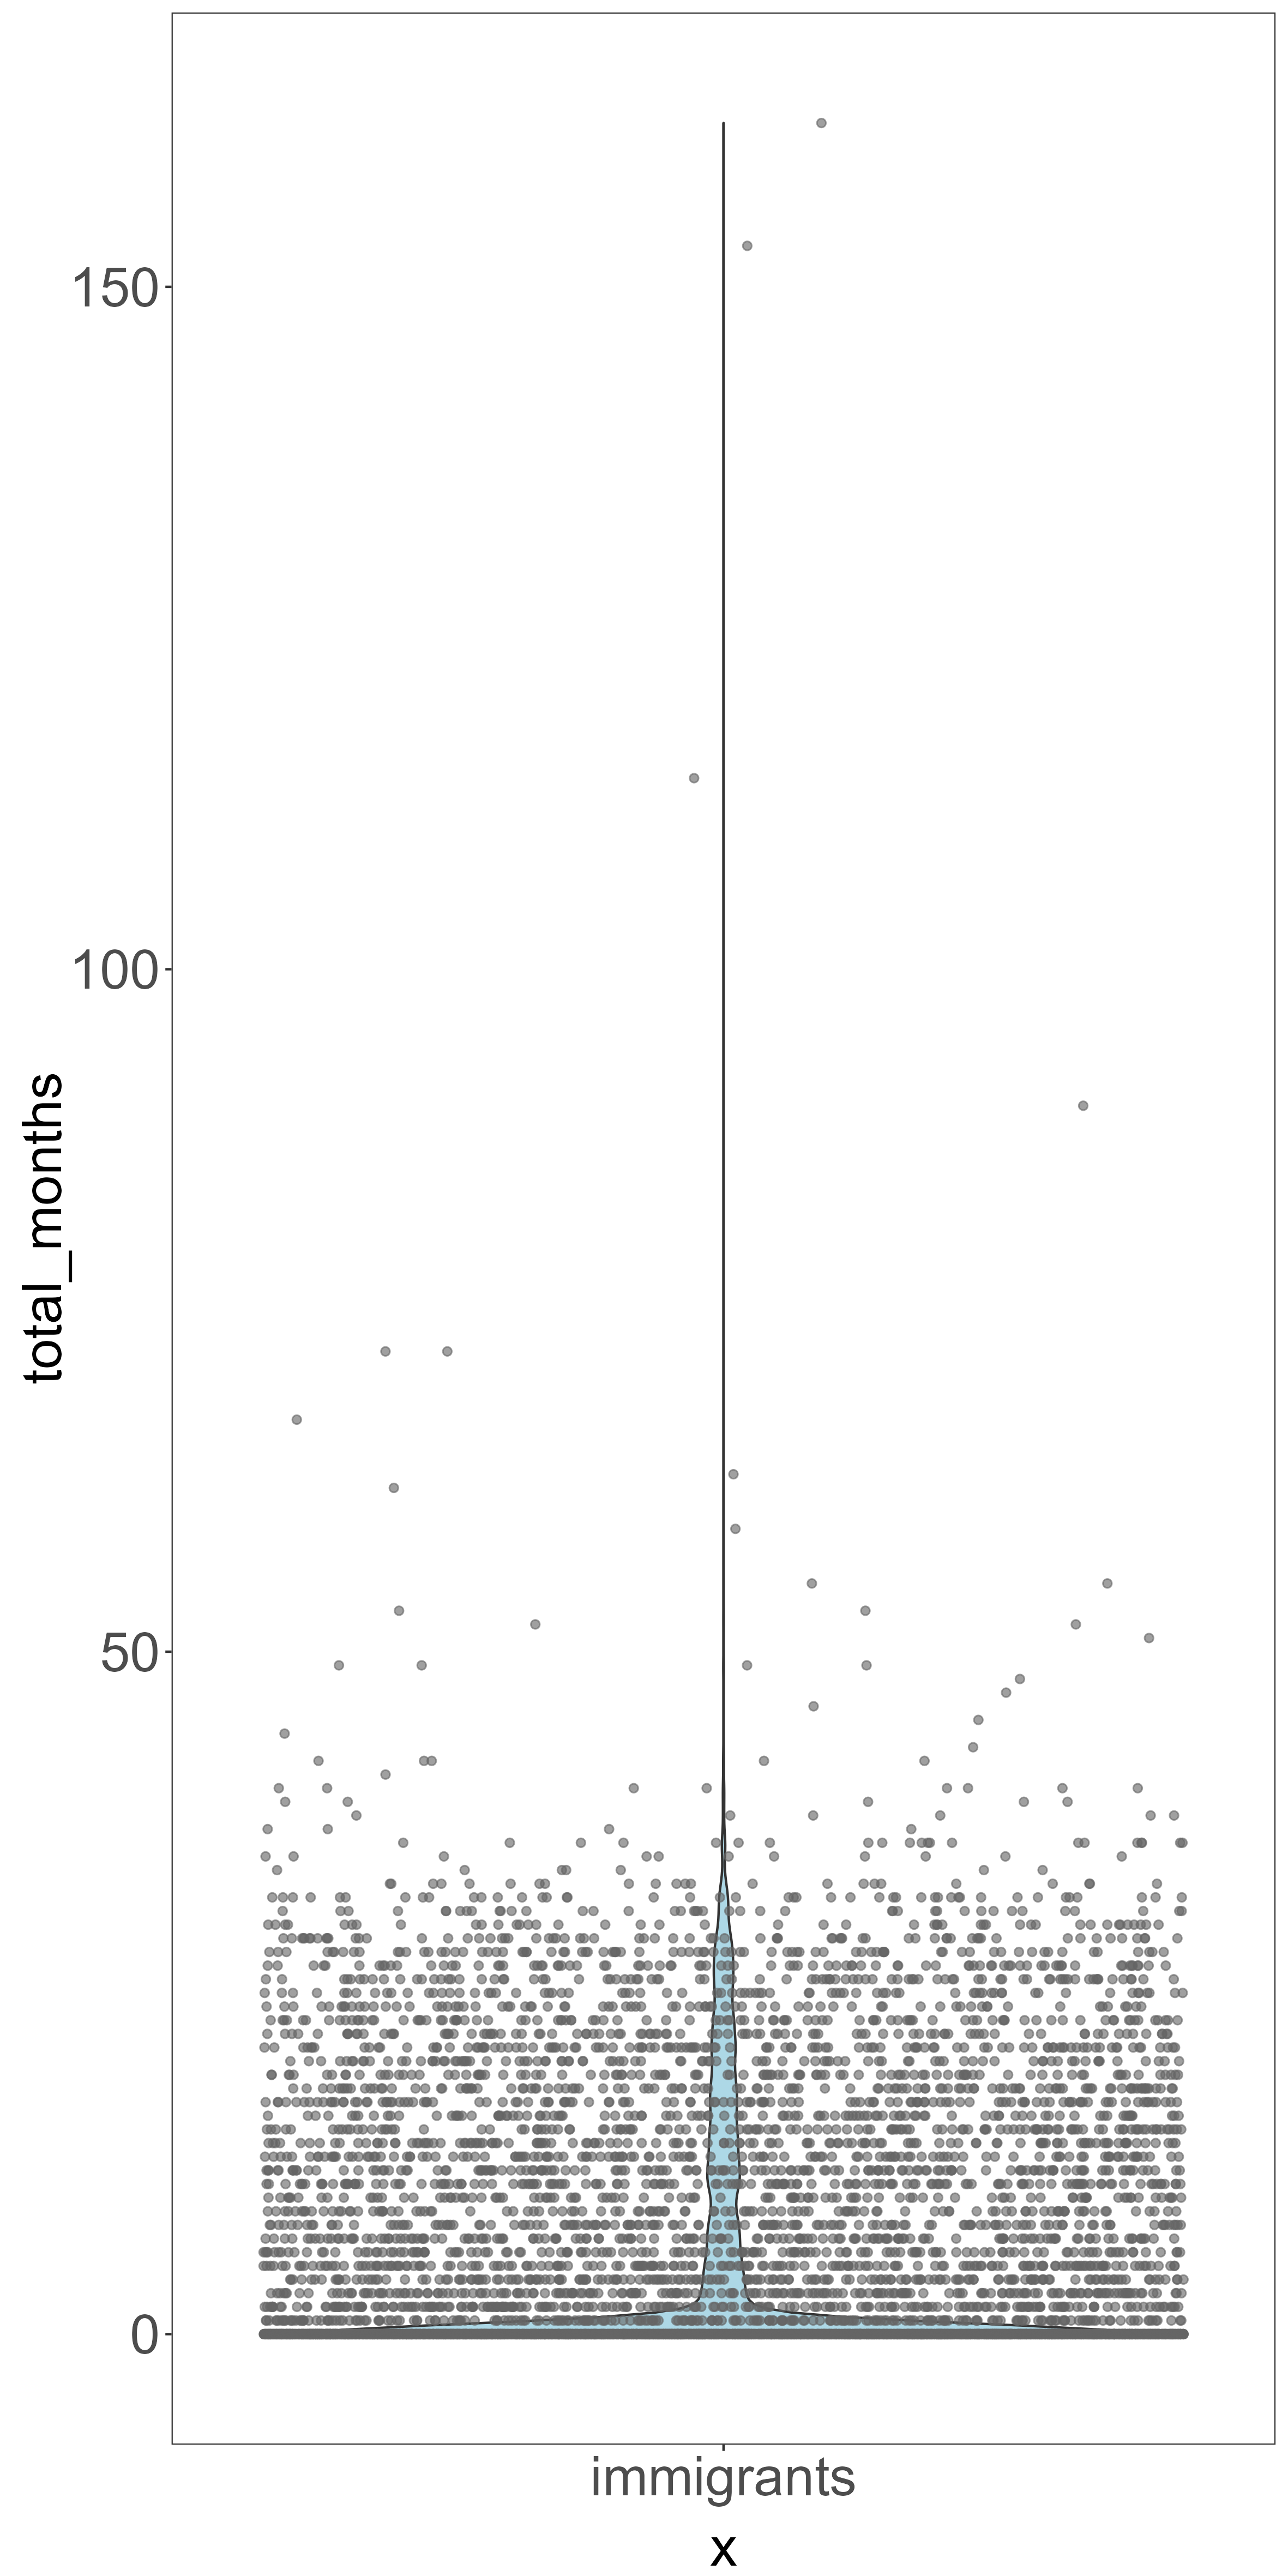
\includegraphics[width=10cm]{total_months_per_pers_violin_plot}
		\caption{Violin plot showing the distribution of months worked by immigrants in the first 3 years, since they entered the country.}
		\label{fig:total_months_per_pers_violin_plot}
	\end{figure}
	
	\section{Question 2:}
	\subsection{Subquestion 1}
	Using OLS, regress various labor market outcomes (female labor participation, female hours of work, total family income) on number of children (our measure of fertility) while controlling for age of the mother, age of mother at first birth, education of the mother and racial variables (i.e., blackm, hispm, othracem). Explain
	why these estimates might not reflect the causal effect of fertility on labor outcomes.
	\subsection{Answer}
	The coefficients of \verb|kidcount| in the model outputs represent the effect of the number of children on the outcome variables \verb|workedm, hourswm, faminc1, incomem| for a one-unit change in the covariate of interest \verb|kidcount|, while the values of the other covariates \verb|agem1, agefstm, educm, blackm, hispm, othracem| are held constant.
	
	Infact, by including all the control covariates in the formula, you are effectively controlling for their effects on the outcome variable, and you will be able to assess the specific impact of "kidcount" on the labor market outcomes while considering the influences of the other covariates.
	
	For example, in all 4 models where we use various labor market outcomes, the coefficient of \verb*|kidcount| is negative. This means that an additional child reduces the probability of working. This may be an intuitive result, but it might not reflect the causal effect of fertility on labor outcomes for the following reasons:
	\begin{enumerate}
		\item Reverse Causality: While you are interested in exploring the impact of fertility on labor outcomes, it's also possible that labor outcomes might affect fertility decisions. For instance, a woman's with a higher income may be more inclined to have one more child because she has better chances to provide for him/her.
		\item Cultural and Societal Factors: Fertility decisions are influenced by complex cultural, societal, and personal factors that might be partially captured by the racial variables, but those covariates may not fully capture the culture and traditions from their specific birth town.
	\end{enumerate}
	
	Some results of the models are worth mentioning:
	\begin{enumerate}
		\item The coefficient of kidcount is negative for all labor market outcomes, with a small std. deviation, so the effect of an additional child is consistently negative across the different outcomes.
		\item The coefficient of kidcount is statistically significant for all labor market outcomes.
		\item In the last 2 models (faminc1 and incomem), the coefficients of `blackm` and `hispm` have opposite sign between the two models. Particularly, the	coefficients of `blackm` and `hispm` are positive in the model for `incomem` and negative for `faminc1`. This may be interpreted as follows: the income of the mother is higher when she is black or hispanic, but the income of the family is lower when the mother is black or hispanic.
		On the other hand, this causal effect is not proven because this may also be due to external factors that are not included in the model, such as the	racial variables related to the father.
		For example, considering the fact that interracial marriages are usually less common, if the mother is black, the father may be more likely to be black as well and this is highly related to his income. So the income of the family may be lower because the father is black, not because the mother is black.
	\end{enumerate}
		
	
	\subsection{Subquestion 2}
	
	The treatment we now consider is the birth of a third child and its effect on these labor outcomes. The instrument we are going to use is whether the first two children have the same sex. Explain the reasoning
	for the choice of the instrument. Explain carefully what the treatment parameter is.
	\subsection{Answer}
	As explained in the previous subquestion 1, the models may be affected by reverse causality, which may hinder the causal interpretation of the results. 
	For this reason, an instrumental variable may help study the causal impact of the birth of a third child. 
		
	Particularly, the binary covariate describing "whether the first two children have the same sex" (\verb|child_same_sex|) may be a good instrumental variable because:
	\begin{enumerate}
		\item \textbf{Exogeneity:} \verb|child_same_sex| is a random variable that is unlikely to be related to any other covariate or unobserved factor that affects labor outcomes. It is important to note that the validity of the chosen instrumental variable relies on the assumption that the instrument has no direct effect on the labor outcomes except through its impact on the treatment (third-child birth). This is also known as the \textbf{exclusion restriction condition}.
		\item \textbf{Relevance condition:} \verb|child_same_sex| is related to the decision of giving birth to a third child, because if the first 2 children have the same sex, the parents may be more inclined to have a third one, wishing to have children with both sexes, so it can be a good instrumental variable to replace the covariate \verb|third_child_birth|.
	\end{enumerate}
	
	The treatment parameter is the birth of the third child \verb|third_child_birth|, meanly we evaluate whether the labor outcomes changed when comparing the mothers who have given birth to the third child and the ones who have not.
	In order to do this, we filter the dataset in order to analyze only the mothers with: 
	$$\verb|kidcount| \text{== 2 or 3}$$
	We exclude mothers with more than 3 kids because otherwise the birth of the 4th (or 5th or more) child may prevent us from analyzing the sole impact of the birth of the 3rd child and it may introduce endogeneity.
	
	
	\subsection{Subquestion 3}
	
	Assess the relevance of the instrument empirically. Explain what it means for an instrument to be relevant and what happens if this is not the case.
	\subsection{Answer}
	When we regress the ``samesex` on ``kidcount`, while using the controls from 1, we obtain that the coefficient of ``kidcount` is positive and statistically significant, so the instrument is relevant.
	Moreover, we notice that the coefficients of the other covariates (that	we used as controls in 1.) are not statistically significant ($\text{p-value}> 0.02$), except for \verb|agem1| and \verb|agefstm|, which have a coefficient that is much smaller than the coefficient of \verb|kidcount|:
	\begin{equation}
		\frac{\beta_{\text{kidcount}}}{\beta_{\text{agefstm}}} = 20.452
	\end{equation}
	so we can conclude that the instrument is not related to the other covariates.
	Furthermore, we can check instruments' relevance by employing the t-test statistics:
	$$t = \frac{\hat{\beta_{\text{kidcount}}}}{\hat{se}(\hat{\beta_{\text{kidcount}}})} $$
	This can test the null hypothesis of non relevant instrument:
	$$H_0 : \beta_{\text{kidcount}} =0$$
	where $\beta_{\text{kidcount}}$ is the coefficient of the instrumental variable.
	In our case we have:
	$$t = \frac{\hat{\beta_{\text{kidcount}}}}{\hat{se}(\hat{\beta_{\text{kidcount}}})} = \frac{0.0804758}{0.0022864} = 35.1976$$
	So, based on the rule of thumb where t should be higher (or equal) than 10.2, we can conclude that the instrument is relevant.
	
	If the instrument was not relevant, the coefficient of \verb|kidcount| would be close to 0 and not statistically significant. In this case, the instrument would not be useful to estimate the causal effect of the treatment (third-child birth) on the outcome.
	Particularly, in finite sample case the 2SLS estimator is biased, but asymptotically (with an infinitely large sample) with relevant instruments the estimator distribution is normal and unbiased. On the contrary, when we have \textit{weak} instruments (not highly relevant or informative), the asymptotic theory is a bad approximation of the finite sample	estimator, so it remains biased, even with large samples.
	
	\subsection{Subquestion 4}
	Estimate by 2SLS the effect of the treatment using the controls from 1. and compare to the OLS estimates. Briefly justify your choice of standard errors.
	\subsection{Answer}
	I choose to use the errors of the 2SLS model, in the "just-identified" case since K="number of endogenous variables" is equal to L = "number of exogenous variables (including instruments)".
	These errors are also called robust/sandwich estimator because there are more robust to
	heteroskedasticity.
	On the other hand, I checked the residuals for heteroskedasticity (see Fig. \ref{fig:2sls_residuals}).
	
	\begin{figure}[H]\centering
		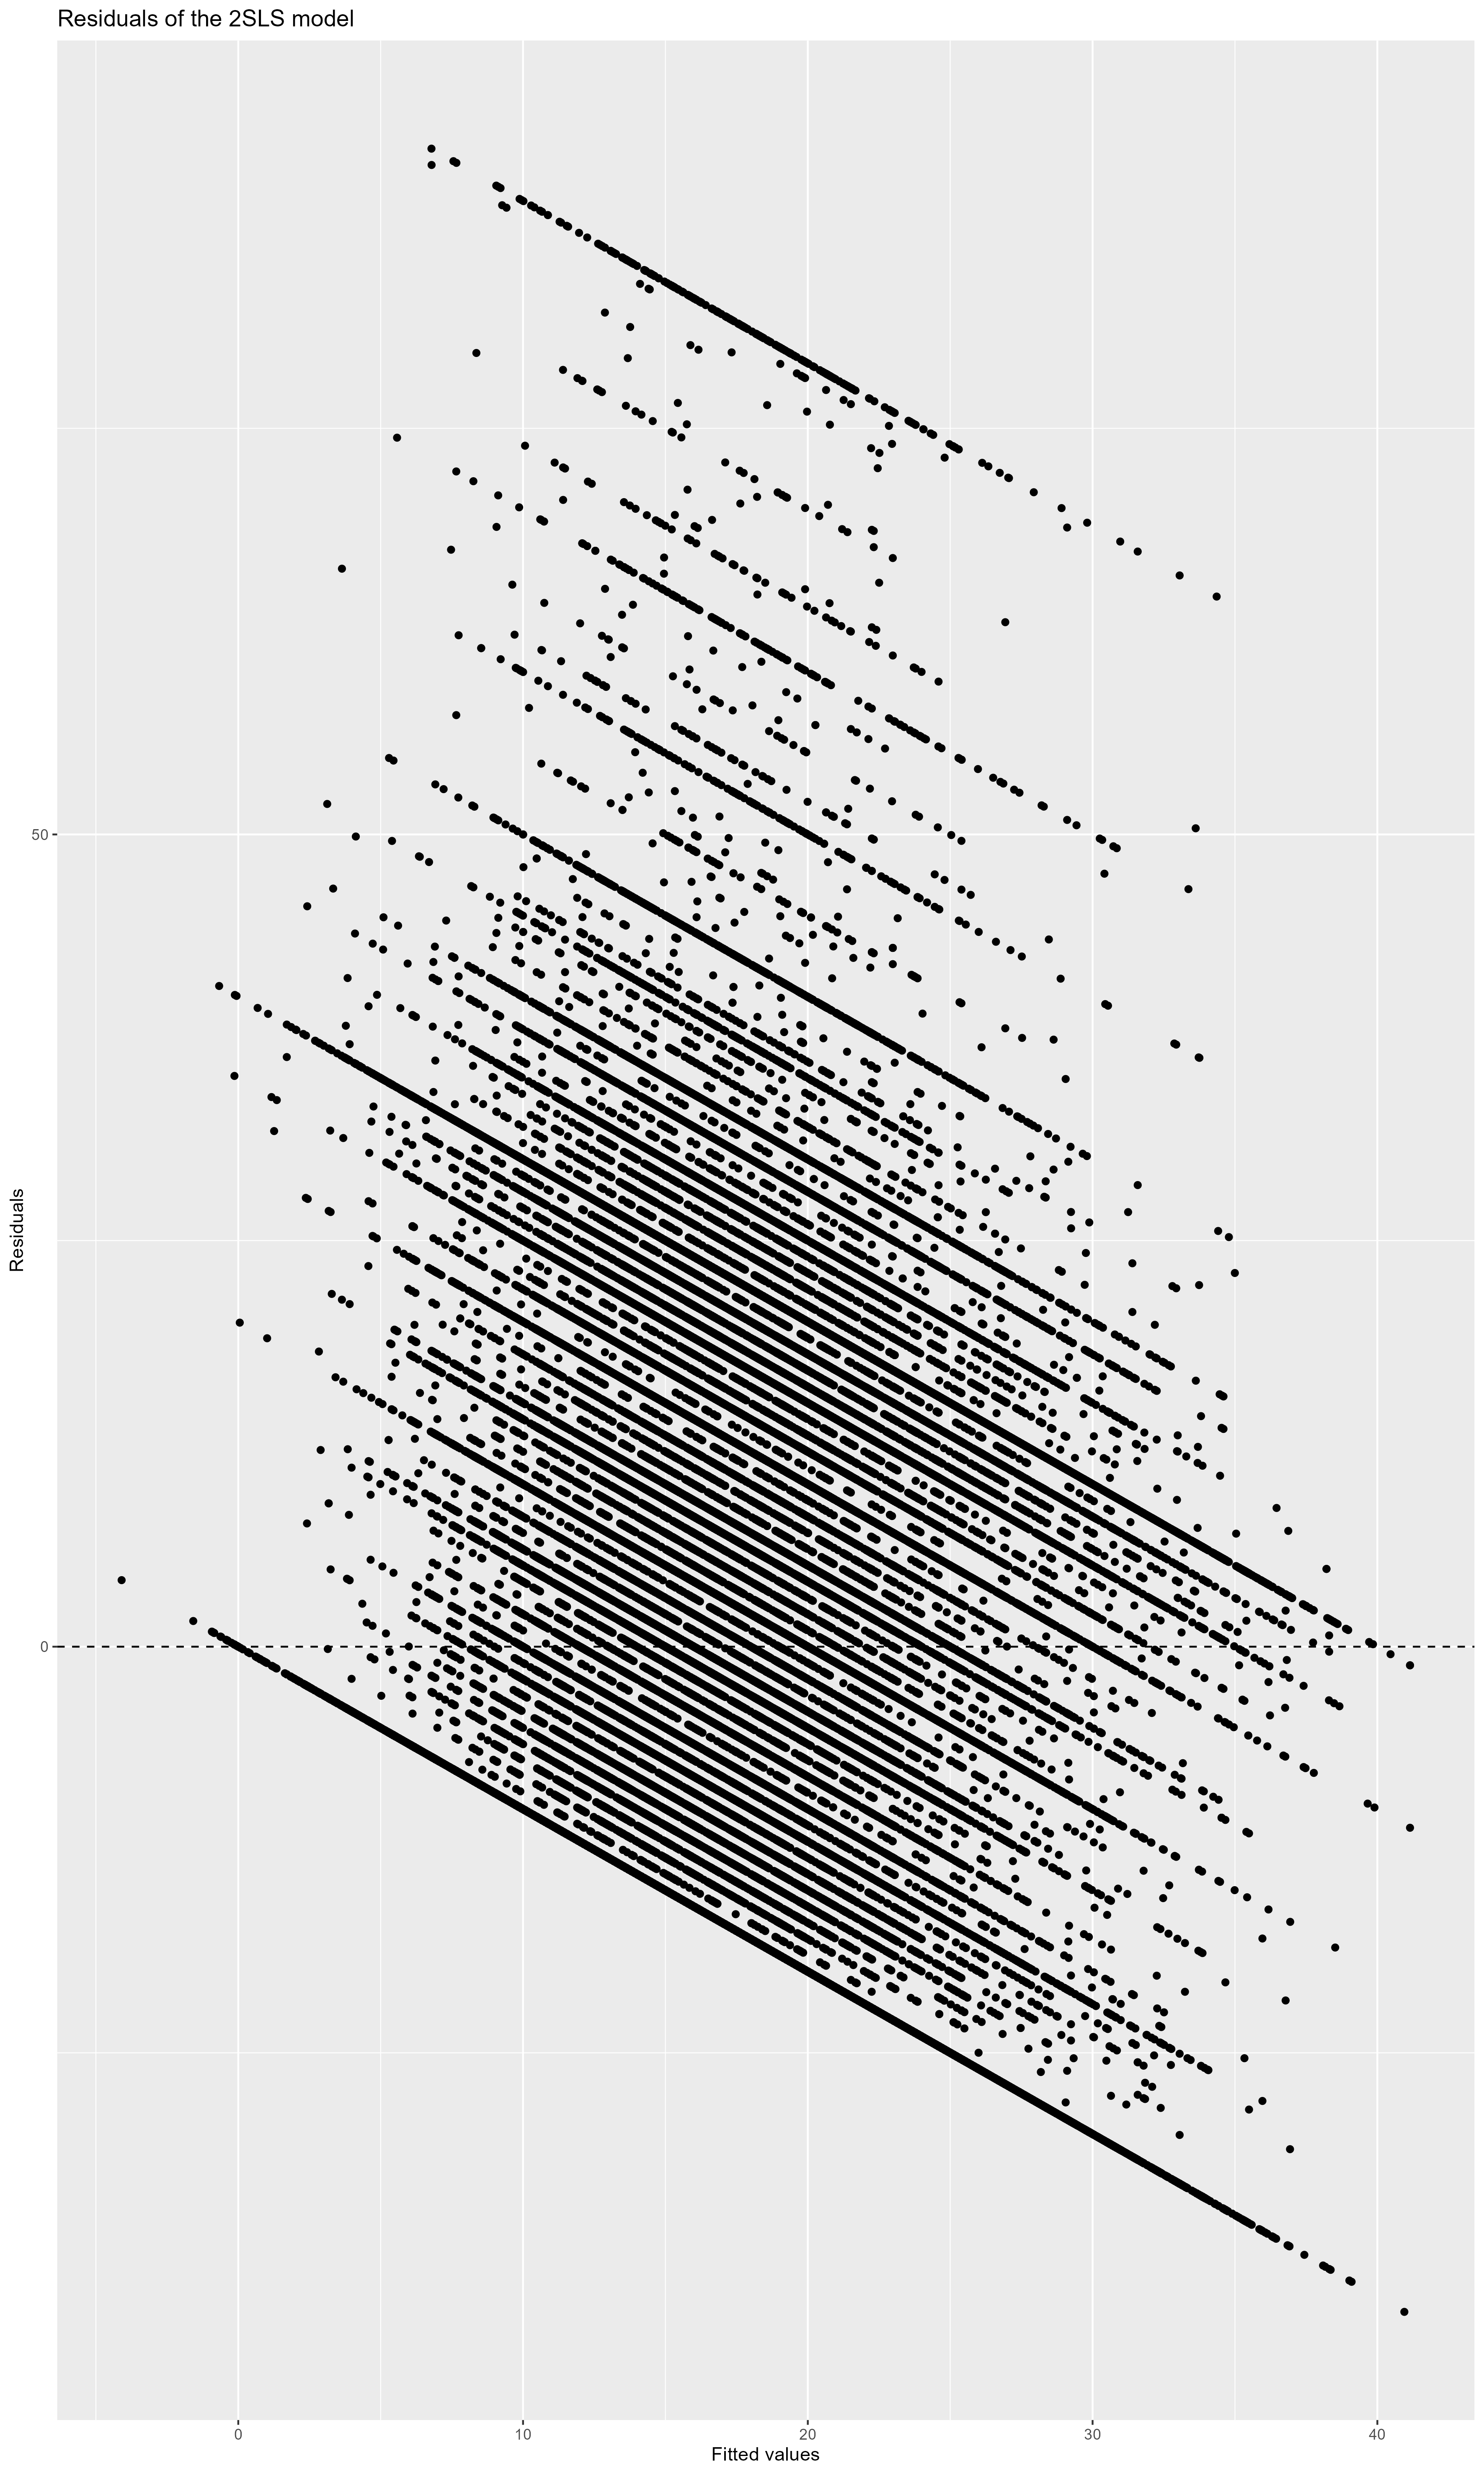
\includegraphics[width=10cm]{2sls_residuals}
		\caption{Residuals of the 2SLS model with target="hourswm".}
		\label{fig:2sls_residuals}
	\end{figure}
	
	\subsection{Subquestion 5}
	NOTE: I did not manage to make my implementation of 2SLS work with more than 10K samples because of memory constraints when creating the projector $P_z$.
	
	\section{Question 3}
	\subsection{Subquestion 1}
	Load the data from PVW\_synth.csv. Set the randomization seed at the beginning of your script to ensure that we can replicate your results. Randomly split the data in (approximately) two halves. The first half is the training sample, the other half is the validation sample.
	\subsection{Answer}
	See the attached code script \verb|question3.R|.
	
	\subsection{Subquestion 2}
	
	\paragraph{LASSO regression}
	LASSO (Least Absolute Shrinkage and Selection Operator) regression is a linear regression technique used for variable selection and regularization. It aims to prevent overfitting in predictive models by adding a penalty term to the linear regression cost function. This penalty term is based on the absolute values of the coefficients of the regression variables.
	
	In LASSO regression, the objective is to minimize the sum of the squared differences between the actual and predicted values, like in ordinary least squares (OLS) regression. However, LASSO adds a constraint on the sum of the absolute values of the coefficients, forcing some of them to be exactly zero. Therefore, the function to minimize (or \textit{"loss function"}) is:
	\begin{equation} \label{eq:lasso_loss}
		\min_{\beta} \left\{ \frac{1}{2n} \sum_{i=1}^{n} (y_i - \beta_0 - \sum_{j=1}^{p} x_{ij}\beta_j)^2 + \lambda \sum_{j=1}^{p} |\beta_j| \right\}
	\end{equation}
	where the first term in the minimization equation represents the ordinary least squares (OLS) loss, while the second term is the L1 regularization penalty.
	
	This results in a sparse model where only a subset of the original variables are retained, effectively performing variable selection.	
	The degree of regularization in LASSO is controlled by a parameter, denoted in Eq.\ref{eq:lasso_loss} as $\lambda$. Larger values of $\lambda$ lead to heavy penalization, meanly an increase in model sparsity with more coefficients being shrunk to zero, which implies less variance but a higher bias. On the other hand, lower values of $\lambda$ lead to higher variance.
	
	LASSO regression is particularly useful when dealing with high-dimensional datasets with potentially many irrelevant or redundant features, as it helps improve model interpretability and generalization by focusing on the most important predictors.
	
	\paragraph{Random Forest}
	Random Forest leverages an ensemble approach by constructing multiple decision trees during training. Decision trees can capture non-linear relationships in the data, but they have high variance, meanly they are  prone to overfitting, especially when they are grown deep with many branches and leaves. This means that they are very unstable and sensitive to small changes in the training data, and they may perform poorly on unseen data.
	For this reason, random forests employ the "bagging" algorithm, which introduces randomness into each tree by using a different bootstrap sample of the whole dataset to train each tree. For this reason, the final prediction is the average value of the prediction of each tree, smoothing out individual tree errors, enhancing robustness and reducing overfitting. In a Random Forest algorithm with N trees, the final prediction of a sample with covariates $W_k = \omega$ is defined as the weighted average of the tree predictions $Y_i$, where the weight is the share of trees predicting $Y_i$ given the sample $W_k = \omega$:
	\begin{equation}
		\hat{\theta}(\omega)= \sum_{i=1}^{N} \frac{\textbf{1}_{T(W_i)=T(\omega)}}{\sum_{j=1}^{N}\textbf{1}_{T(W_j)=T(\omega)}} * Y_i
	\end{equation}
	For these reasons, Random Forest algorithm improves generalization, enhances the model's ability to handle non-linearities in data, and it can also provide feature importance insights.
	
	\subsection{Subquestion 3}
	Fit these learners to the training sample using net financial assets as the outcome and using the predictors listed above. Briefly motivate your choice of (hyper)tuning parameters.
	\subsection{Answer}
	I fit LASSO model with multiple values of lambda, in order to look for the optimal one, and I obtained the plot \ref{fig:MSE_vs_lambda}. In the plot we see that when the lambda value has certain values, the MSE does not change, because either all the regressors are being considered (left-side of the plot) or none of them (right-side). Therefore, we choose the lambda that can keep a low MSE, while reducing model complexity (variance), which is:
	$$\lambda =  533.670$$
	which in the graph corresponds to the left dashed line ($Log(533.670)=6.279$).
	Moreover, fig. \ref{fig:coefficients_vs_lambda} shows how the coefficient of the regressors change for different lambda values. We can notice that at higher lambda values, more coefficients go to zero, leading to a lower variance, but a higher bias. Infact, we 
	also notice that for $$Log(\lambda_{optimal}) = 6.279$$ many regressor coefficients are set to zero, which indicates that the other regressors are not relevant to predict "net total financial assets".
	\begin{figure}[H]\centering
		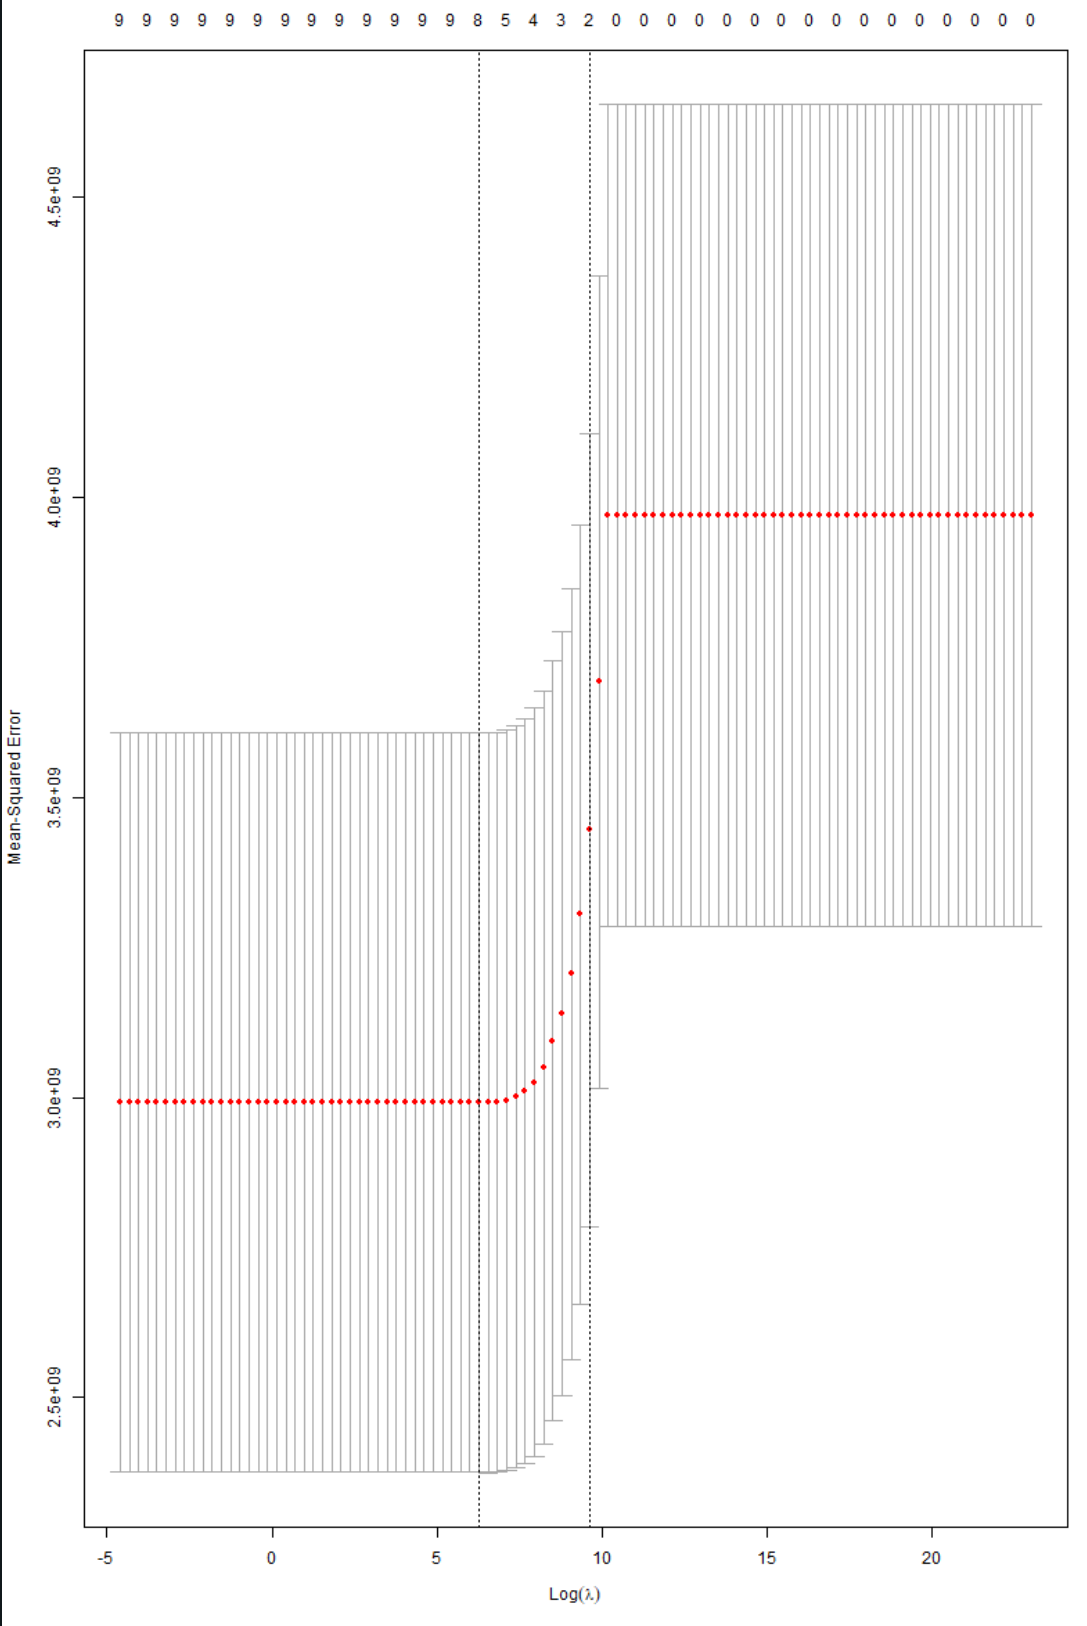
\includegraphics[width=10cm]{MSE_vs_lambda}
		\caption{Value of the Mean Squared Error when varying the lambda value. The left dashed line indicates the optimal lambda value}
		\label{fig:MSE_vs_lambda}
	\end{figure}

	\begin{figure}[H]\centering
		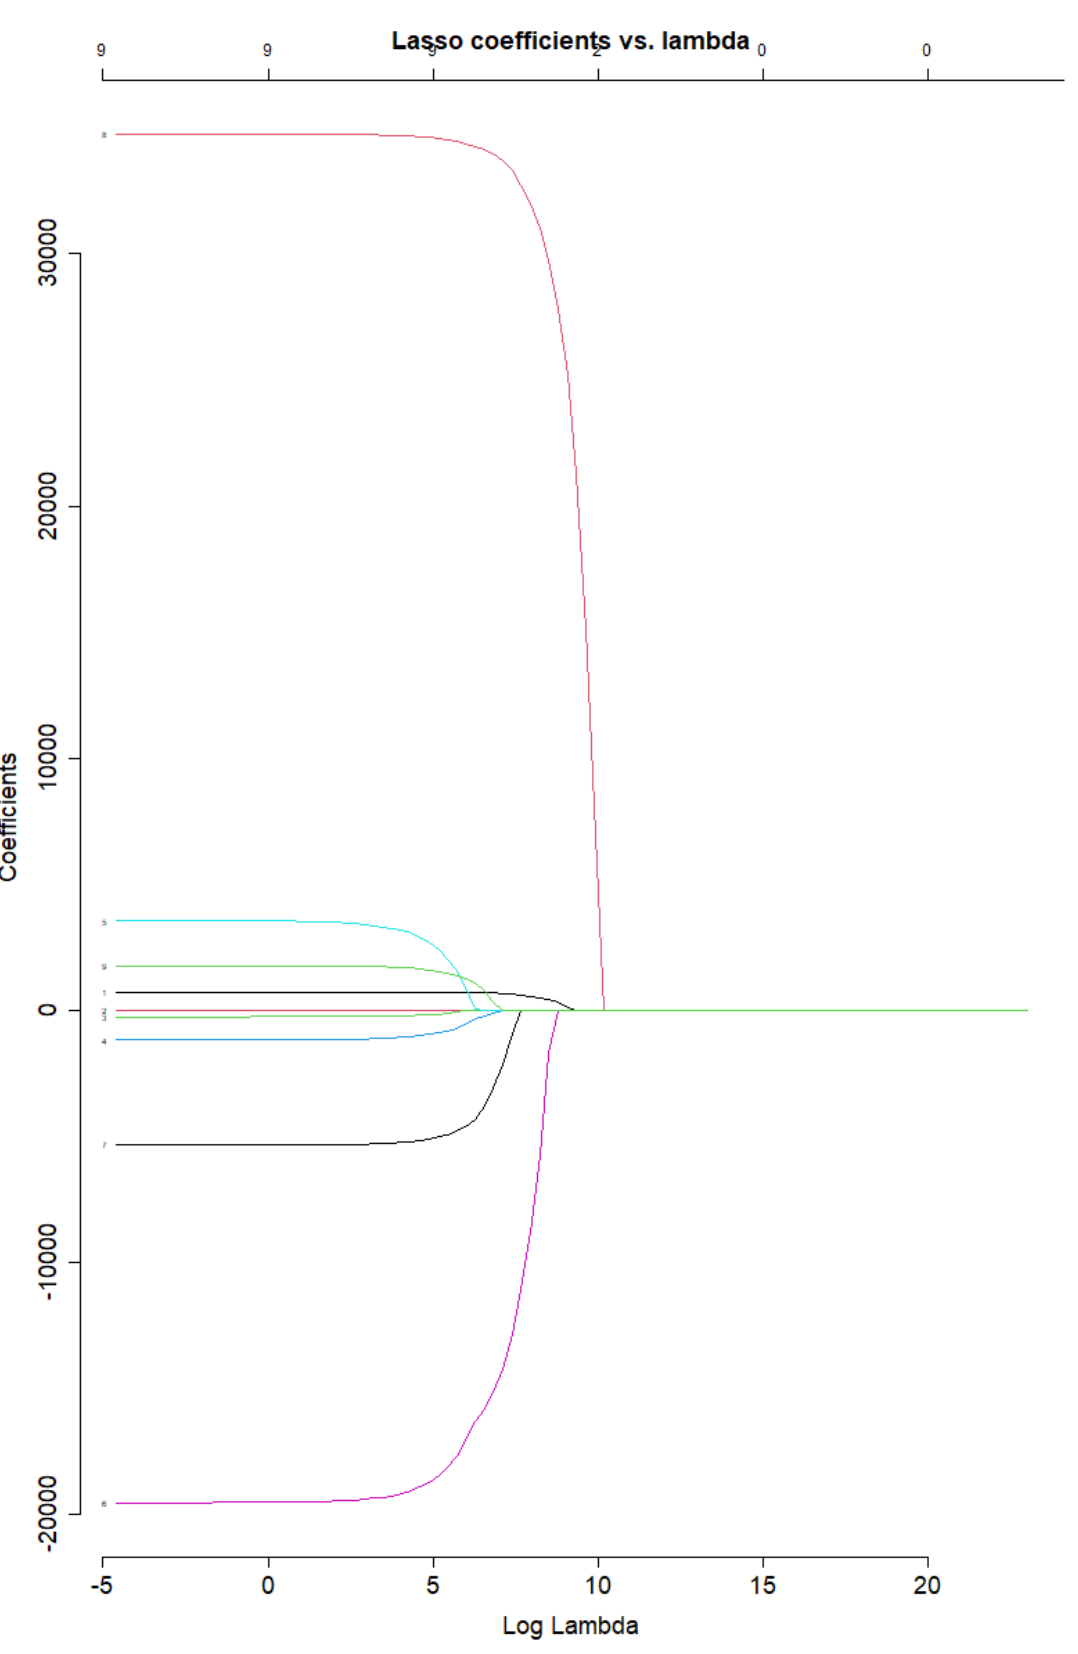
\includegraphics[width=10cm]{coefficients_vs_lambda}
		\caption{Regressor coefficient values for multiple lambda values.}
		\label{fig:coefficients_vs_lambda}
	\end{figure}

	Similarly, I tried multiple combinations of 2 parameters of the Random Forest algorithm in order to identify which one can minimize the error:
	\begin{itemize}
		\item \textbf{Number of variables used at each split} \verb|mtry|. When each branch of the decision trees of the Random Forest is created, only a subset of regressors is randomly sampled as candidates to define the 2 branches. The random sampling of the covariates introduces more randomness among the decision trees, in order to prevent that one regressor dominates the branch creation. 
		For these reasons, a large value may lead to more instability and higher variance because it decreases randomness among trees.
		The recommended value is \verb|mtry = p/3| for regression tasks (and $sqrt(p)$ for classification tasks), where \verb|p| is the number of regressors. In our case, we have 9 regressors, so I choose is \verb|mtry = 3|.
		\item \textbf{Number of trees to grow} \verb|ntree|. This controls the number of trees of the Random Forest. If this is set to a small number, it is more likely to have higher bias and lower performances on the train set. On the contrary, a high number of trees leads to higher computation time and complexity, along with the risk of overfitting, higher variance, and a lower performance on the validation set.
	\end{itemize}
	
	In order to choose the values of these parameters, I split the training set into two subsets (80/20 ratio), called \verb|subtraining_data| and \verb|subvalidation_data|. Then I ran the Random Forest algorithm with multiple combinations of both values and I compared the MSE computed on \verb|subvalidation_data| (see figure \ref{fig:RF_error_vs_mtry_ntree}).
	
	\begin{figure}[H]\centering
		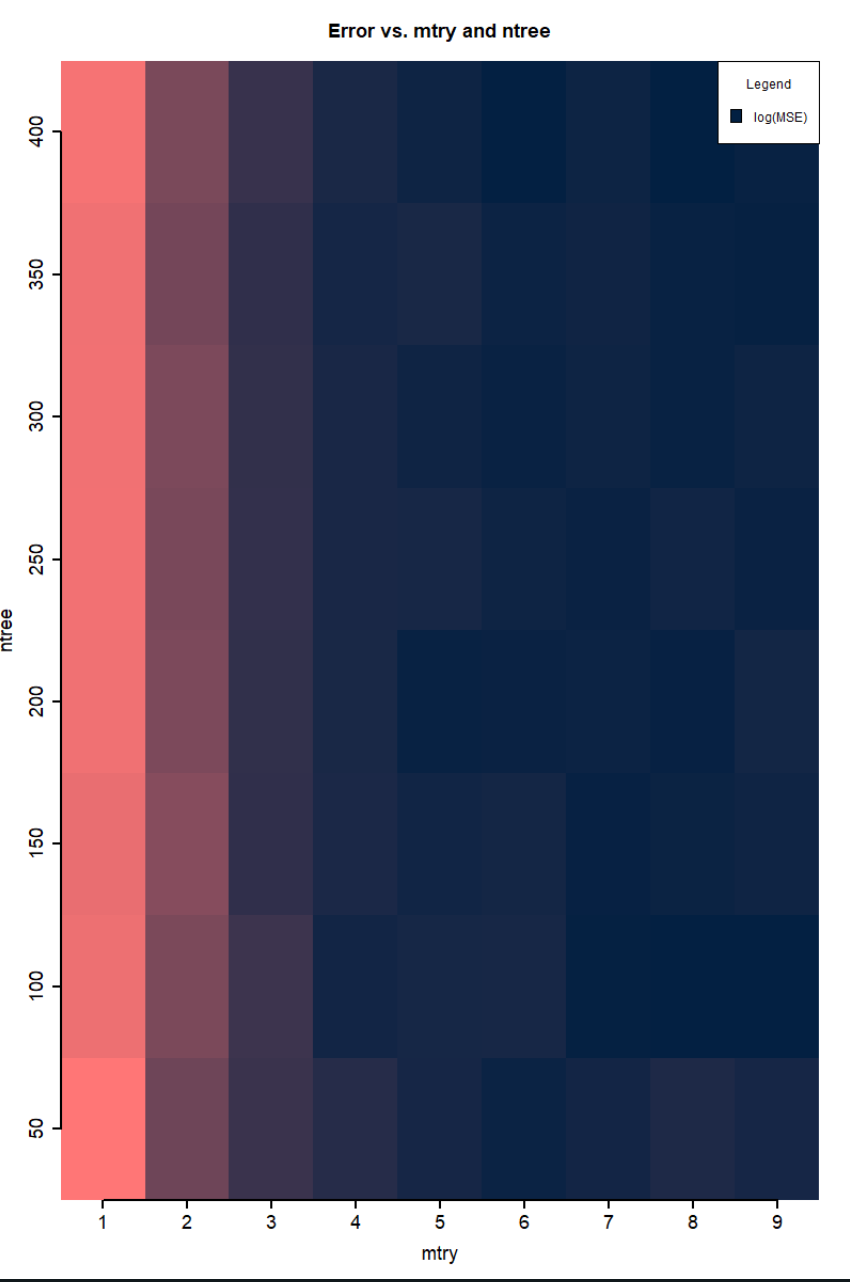
\includegraphics[width=10cm]{RF_error_vs_mtry_ntree}
		\caption{Heatmap of the Mean Squared Error (logarithm scale) computed for multiple combinations of the two parameters "(ntree, mtry)".}
		\label{fig:RF_error_vs_mtry_ntree}
	\end{figure}
	 
	Since there are multiple combinations \verb|(ntree, mtry)| with similarly low errors, we choose the lowest values of \verb|ntree| and \verb|mtry| that minimize the validation error, in order to prevent overfitting, while maintaining a low bias, meanly:
	\verb|(ntree, mtry)| = (100, 4) .
	
	\subsection{Subquestion 4}
	Assess the relative prediction performance of lasso and random forests using the validation sample. (Short statement.)
	\subsection{Answer}
	I compared the prediction performance of LASSO and Random Forest by computing the MSE on the validation set and I obtained:
	$$MSE_{LASSO}=3530464334$$
	$$MSE_{RF}=1812446656$$
	
	To compute $MSE_{LASSO}$, I employed the best lambda value, which is the value that minimize the loss function of LASSO algorithm (Eq. \ref{eq:lasso_loss}).
	The MSE comparison shows that Random Forest has better performances than LASSO on the validation set, which contains a subset of data that was not used to fit the models.
	Generally speaking, LASSO aims at reducing the dimensionality of datasets with many regressors, especially when there is a strong multiple collinearity. On the contrary, Random Forest has better performances when there are non linearities in the dataset. This could be the case of \verb|education|, \verb|income| or boolean variables like "home ownership", "being married" or "having a second positive income". These variables may imply discontinuities or rapid changes in the "net total financial assets", and this could be one of the reasons of the better performances of Random Forest algorithm.
	On the other hand, a more robust and popular approach to compare models employs the Cross-Validation approach where the dataset is split into N=5 or N=10 mutually exclusive folds. Then for each fold the model is trained on the N-1 remaining folds and evaluated on that fold. This approach, although more computationally expensive, has the advantage that the models are evaluated on the whole dataset, in order to have a more reliable evaluation of the model performances.
	
	\section{Question 4: White flight}
	In a recent working paper, Bayer et al. study if households are more likely to move away if a neighbor of different race moves into the same neighborhood. The study thus attempts to shed lights on the drivers of segregation. Explain why it is challenging to identify the causal effect of a new arrival in a neighborhood on the probability of other-race households to move away, and explain how Bayer et al. tackle this task. (Please do not use more than
	250 words. Note that this question requires no estimation.)
	\subsection{Answer}
	[Unfortunately, I had not enough time to complete this question]
	
	\newpage
	
	
\end{document}

									
